\documentclass{standalone}
\usepackage{tikz}
\usepackage{amsmath}

\begin{document}

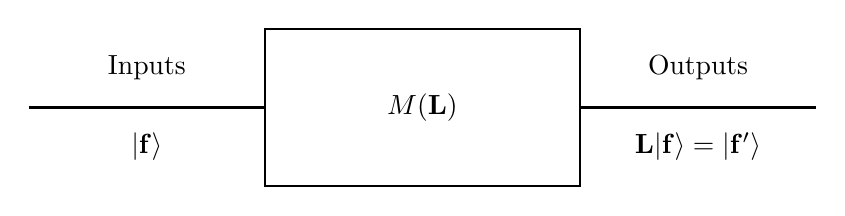
\begin{tikzpicture}

  % Draw the box
  \draw[thick] (0,0) rectangle (4,2);
  
  % Draw the input line
  \draw[thick] (-3,1) -- (0,1);
  
  % Draw the output line
  \draw[thick] (4,1) -- (7,1);
  
  % Input label
  \node at (-1.5, 1.5) {Inputs};
  \node at (-1.5, 0.5) {$|\mathbf{f}\rangle$};
  
  % Output label
  \node at (5.5, 1.5) {Outputs};
  \node at (5.5, 0.5) {$\mathbf{L}|\mathbf{f}\rangle = |\mathbf{f'}\rangle$};
  
  % Box label
  \node at (2, 1) {$M(\mathbf{L})$};
  
\end{tikzpicture}

\end{document}